\chapter{La matemática detrás del Póker: Combinatoria y Probabilidad}

\section{Probabilidad de las jugadas}
\label{sec:prob_jug}

Durante las partidas de Texas Hold’em, los jugadores tratan de obtener una jugada que resulta de combinar de cinco cartas de entre toda la baraja, resultando en un caso de combinatoria. Esto se traduce en 52 posibles cartas escogidas 5 cartas sin importar el orden y sin repetición, por lo cual se obtiene un total de $\binom{52}{2}$ = 2.598.960 posibles combinaciones. 

Partiendo de la tabla \ref{tab:jugadas}, es posible calcular las probabilidades de obtener cada tipo de jugada dividiendo el número de posibilidades entre el número de casos completos.Hay que tener en cuenta varias cosas en lo que se refiere a la baraja:
\begin{itemize}
\item El Texas Hold'em utiliza una baraja francesa estándar, por lo que la baraja contiene 52 cartas
\item Cada carta tiene la misma posibilidad de aparecer que el resto de cartas restantes del mazo.
\end{itemize}

Con esto, se puede obtener también la cuota de esa mano también conocida como \textit{odds}, que es el inverso de la probabilidad. La cuota define el el ratio de la cantidad de manos que no son la buscada.
Por ejemplo, el número de Escaleras de color posibles son 36, por lo que se puede calcular el número de casos que no son una Escalera de color (2.598.960-36=2.598.924), por lo que la cuota sería 2.598.924:36, que simplificando es 72.192,3:1.

Las cuotas se tratarán en profundidad en el apartado \ref{sec:odd}.

Ahora se procede a calcular la tabla con la probabilidad de cada una de las manos.

\begin{longtable}[c]{|c|m{4em}|m{8em}|c|c|c|}
\hline
\rowcolor{lightgray} Orden & Nombre & Ejemplo &  N & Prob(\%) & Cuota\\ \hline
1 & Escalera Real \textit{Royal Flush}&\textcolor{red}{A$\varheartsuit$K$\varheartsuit$Q$\varheartsuit$J$\varheartsuit$10$\varheartsuit$}& 4 &$1.539*10^{-4}$&649.739:1\\
\hline
2 & Escalera de Color \textit{Straight flush}&$\clubsuit$8$\clubsuit$7$\clubsuit$6$\clubsuit$5$\clubsuit$&36& $1,385*10^{-3}$&72.192,3:1\\
\hline
3 & Póker \textit{ Four of a kind}& \textcolor{red}{7$\varheartsuit$7$\vardiamondsuit$}7$\clubsuit$7$\spadesuit$2$\clubsuit$ & 624 & $2.4001*10^{-2}$&4.164:1 \\
\hline
4 & Full \textit{Full House}&6$\clubsuit$6$\spadesuit$\textcolor{red}{6$\vardiamondsuit$10$\varheartsuit$}10$\clubsuit$ &3.744&$0,1441$&693,2:1 \\
\hline
5 & Color \textit{Flush} & \textcolor{red}{K$\vardiamondsuit$8$\vardiamondsuit$7$\vardiamondsuit$6$\vardiamondsuit$4$\vardiamondsuit$} & 5.108 &$0,1965$& 507,8:1\\
\hline
6 & Escalera \textit{Straight}&\textcolor{red}{Q$\vardiamondsuit$J$\varheartsuit$}10$\clubsuit$9$\spadesuit$8$\clubsuit$ &10.200& $0,3924$&253,8:1 \\
\hline
7 & Trío \textit{Three of a kind}&\textcolor{red}{7$\varheartsuit$7$\vardiamondsuit$}7$\clubsuit$K$\spadesuit$2$\clubsuit$& 54.912 &$2,1128$&46,3:1 \\
\hline
8 & Doble Pareja \textit{Two Pair}& 8$\spadesuit$8$\clubsuit$6$\spadesuit$\textcolor{red}{6$\varheartsuit$2$\vardiamondsuit$}& 123.552 & $4,7539$&20,03:1\\
\hline
9 & Pareja \textit{Pair}& 7$\spadesuit$7$\clubsuit$K$\spadesuit$\textcolor{red}{4$\varheartsuit$}2$\spadesuit$  & 1.098.240 & $42,257$&1,366:1 \\
\hline
10 & Carta Alta\textit{High Card}&\textcolor{red}{A$\varheartsuit$}10$\spadesuit$8$\clubsuit$7$\spadesuit$2$\clubsuit$ & 1.302.540 & $50,1177$&0,995:1 \\
\hline
\caption{Probabilidad de Jugadas en Texas Hold'em}
\label{tab:prob_jugadas}
\end{longtable}


\section {Cuotas implícitas y Cuotas de Bote}
\label{sec:odd}

A la hora de definir una estrategia, es decir, a la hora de decidir qué decisiones tomar, se tienen numerosos factores a tener en cuenta. En el Texas Hold’em, es tremendamente difícil especificar una estrategia, debido a la cantidad de posibles caminos combinatorios (1326 posibles manos iniciales, 19600 posibles combinaciones de 3 cartas en el Flop, 47 cartas en Turn y 46 para River). Incluso factorizando por palos, siguen quedando más de 5 millones de combinaciones mesa/mano para tener en consideración. 

Para poder definir una estrategia, es necesario considerar varios factores. En la sección \ref{sec:bluff}, se introdujeron los conceptos de de \textit{draw} y \textit{made hand}, que son algunos de esos factores a considerar.

En la sección \ref{sec:prob_jug} se hizo una introducción de otro de esos factores: la cuota. La cuota de una jugada es el ratio de no encontrar la mano buscada. Es decir, es la diferencia del total de combinaciones y las combinaciones del tipo que se busca. Esta cuota también se la conoce como cuota en contra. Pero no es la única cuota relacionada con el póker.

Otra de las cuotas que tienen relevancia a la hora de definir una estrategia es la cuota de bote o \textit{pot odds}. Esta cuota se define como el ratio de diferencia de tamaño entre la apuesta total de una ronda de juego con la apuesta de un jugador. Es decir, cuántas veces es más grande el bote si se compara con la apuesta. Esta cuota es el inverso del cociente de la apuesta del jugador entre la apuesta total.\cite{chen}

Poniendo un ejemplo, si el Jugador A ha apostado 20 €, el Jugador B ha apostado 60€ y el bote suma 80€, la cuota de bote del jugador A sería $(\frac{20}{80})^{-1}=\frac{80}{20}=4$ mientras que para el jugador B sería  $\frac{80}{60}=1.3333$.

Esta cuota es un valor importante para poder cálcular qué se puede esperar a la hora de apostar. Es decir, si el inverso de la probabilidad de ganar el bote es menor a su cuota de bote. Este factor puede generar mucha información, pero presenta un problema.\cite{chen}

El problema de considerar únicamente las cuotas de bote es que estas cuotas no son fieles al funcionamiento real del póker, ya que los jugadores que tengan  \textit{draw} nunca ganarían dinero una vez que reciben su mano ya que la descartarían en el momento en que vieran que tienen un \textit{draw}, pues si probabilidad de ganar con esa mano es muy baja.

Sin embargo, que un jugador tenga un \textit{draw} puede dar lugar a una estrategia que, en un juego donde hay cartas ocultas, podría llegar a resultar altamente explotable. En otras palabras, el jugador con \textit{draw} puede anticipar información extrayendo valores cuando recibe el \textit{draw}. A la combinación de cuotas inmediatas y valor esperado de fases posteriores de la ronda se le conoce como cuota implícita. \cite{chen}

Poniendo un ejemplo de esto último:  \cite{chen}

Jugador A: \textcolor{red}{A$\vardiamondsuit$K$\vardiamondsuit$}

Jugador B: 8$\clubsuit$ 7$\clubsuit$

Flop: A$\clubsuit$ K$\spadesuit$ 4$\clubsuit$

Bote preflop: 135 €

Apuesta del jugador A en Flop: 30€

Límite de apuesta: 30-60€

Se puede observar que el Jugador A tiene dobles parejas de AK mientras que el jugador B tiene un \textit{draw} de Color, a falta de una carta de $\clubsuit$. El jugador A no está seguro si el jugador B tiene \textit{draw} o no, pero se asume que el jugador A verá las apuestas del jugador B en cada una de las fases para continuar con el ejemplo.

Por tanto, se asume que B ve la apuesta de A y se continúa a la fase de River, con un total de 195€ en el bote. En este punto hay 3 casos posibles:
\vspace{5mm} %5mm vertical space

\textbf{Caso 1: La carta revelada en Turn es un trébol.}
\vspace{5mm} %5mm vertical space

 En este caso, el jugador B apostaría la apuesta alta (60€) en cada una de las dos fases posteriores (Turn y River), y el jugador A las vería ambas,tal y como se ha asumido. Esto suma al bote 120€ en cada una de las rondas, que contando los 195€ que tenía el bote tras el flop, el bote total es 435€. Para calcular el beneficio del jugador B, es necesario restarle al bote la cantidad apostada en cada una de las 3 rondas que se conocen(30+60+60 = 150 €), quedando un beneficio de 435-150=285 €. 

En este caso, la probabilidad de que ocurra esta situación es 
p(\textit{Trebol en Turn}) = 8/45 = 0,1778 =17,78\%.

\vspace{5mm} %5mm vertical space
\textbf{Caso 2: La carta revelada en Turn no es un trébol pero la carta revelada en River sí que es trebol}
\vspace{5mm} %5mm vertical space

En este caso, el jugador A apostaría la apuesta alta (60 €) en Turn, el jugador B la vería y en River es el jugador B el que apostaría la apuesta alta y el jugador A la vería. El beneficio sería el mismo que en el anterior caso (285 €).
La probabilidad de que ocurra este caso es la probabilidad conjunta de ambos eventos, es decir
 p(\textit{No trébol en Turn} $\cap$ \textit{Trebol en river}) = p(\textit{No trébol en turn})*p(\textit{Trebol en River}) = 37/45 * 8/44 = 0,1495 = 14,95 \%.


\vspace{5mm} %5mm vertical space
\textbf{Caso 3: Ninguna de las cartas reveladas es un trébol}
\vspace{5mm} %5mm vertical space

En este caso, el jugador A apostaría la apuesta alta (60 €) en Turn, el jugador B la vería, y en River el jugador no vería la apuesta y pasaría, obteniendo un beneficio de -30-60=-90€.
La probabilidad de que ocurra es el opuesto a que ocurra cualquiera de los otros dos casos, es decir\cite{chen}
p(\textit{ningún trébol}) =(37/45)*(36/44) = 1- (8/45 + 37/45*8/44) = 0.6727 = 67.27 \%.

Teniendo estos tres casos, se puede calcular el valor esperado ponderado para cada uno de estos casos, siendo el valor ponderado la multiplicación del valor por la probabilidad. Con esto, se puede elaborar la siguiente tabla:
\begin{longtable}[c]{|c|c|c|c|}
\hline
\rowcolor{lightgray}Salida & p(\textit{Salida}) & Valor (Beneficio) & Valor Esperado Ponderado\\
\hline
Trebol en Turn & 0.1778&+285 €&+ 50,673 €\\
\hline
Trebol en River&0.1495&+285 €&+ 42,6075 €\\
\hline
No trébol&0.6727&-90 €&-60,543 €\\
\hline
Total & 1 & &+ 32.7375 €\\
\hline
\caption{Ejemplo de cuota implícita}
\label{tab:implied}
\end{longtable}

Al sumar los valores esperados ponderados, se encuentra que que esta ronda tiene una expectación de ganar alrededor de 32,74€. Es importante tener en cuenta la cuota implícita cuando tienes una mano con \textit{draw}, ya que hay que tener en cuenta no solo la cantidad que se pueda ganar en caso de que salgan los \textit{outs} necesarios como la cantidad que se pueda perder en caso contrario. Tampoco se puede asumir que nuestros oponentes van a seguirnos el ritmo apostando.\cite{chen}

\section{Teorema de Bayes}
\label{sec:bayes}

El Teorema de Bayes es una herramienta que permite obtener la probabilidad de un evento condicionado en otro cuando se tiene la distribución del otro evento condicionado en ese evento y una distribución marginal de probabilidad del evento buscado. \cite{chen}

Desde el punto de vista del póker, el teorema de Bayes sirve como realimentación para la toma de decisiones y las estimaciones de probabilidad, puesto que, a medida que se vaya obteniendo nueva información, permite reajustar la estimación sobre la probabilidad y las estrategias a seguir. Esto resulta de especial utilidad, en concreto, para leer las manos y las acciones del oponente. 

La clave de la aplicación del teorema de Bayes es la existencia de una probabilidad previa y la obtención de información nueva, revisando y actualizando la probabilidad con la información obtenida. A este proceso se le conoce como inferencia Bayesiana.

De cara a este proyecto, se va a utilizar el teorema de Bayes para intentar identificar a cuál de los patrones predefinidos se enfrenta el algoritmo, y corregir las acciones del mismo según a qué patrón se enfrente.

Se procede a desarrollar la fórmula del teorema de Bayes.\cite{chen}

En el Anexo \ref{ch:AxA}, se define la fórmula genérica de la probabilidad de tener dos eventos simultáneamente:


\[p(A\cap B)=p(A)*p(B | A)\]

Se reorganiza la fórmula para intentar despejar la probabilidad de B condicionado en A:

\[p(B|A)=\frac{p(A\cap B)}{p(A)}\]

También se puede definir la probabilidad de que no ocurra el evento B. En otras palabras, la probabilidad de $\tilde{B}$:

\[p(B) + p (\tilde{B}) = 1 \rightarrow p (\tilde{B}) = 1 - p(B)\]

A partir de aquí, sabiendo que se tiene que cumplir siempre p(B) + p ($\tilde{B}$) = 1, se puede expresar p(A) como la probabilidad de A condicionado en B más la probabilidad de A condicionado en $\tilde{B}$, lo que genera la fórmula del teorema de Bayes:


\[p(B | A) = \frac{p(A|B)*p(B)}{p(A|B)*p(B) + p(A|\tilde{B})*p(\tilde{B})}\]

\section{Clasificación de manos iniciales: Criterio de Sklansky-Malmuth y Fórmula de Chen}
\label{sec:chen}

En el Texas Hold'em, se puede agrupar las decisiones, es decir, las acciones que se toman en las rondas de apuesta, en dos tipos:
\begin{itemize}
\item Decisiones con una jugada ya formada. En otras palabras, teniendo al menos 5 cartas conocidas. Esto corresponde a las rondas Flop, Turn y River.
\item Decisiones sin una jugada formada, es decir, teniendo las 2 cartas iniciales (Preflop).
\end{itemize}

Para las apuestas del primer tipo, se disponen de muchos elementos, factores y más información sobre la estrategia a seguir, el potencial de la jugada, las probabilidade sde tener mejor jugada y cuántos jugadores quedan en la partida. Pero para las apuestas del segundo tipo, la cantidad de información es mucho más limitada, por lo que es necesario aplicar otro criterio para la toma de decisiones.

Uno de los criterios más extendidos, y que se va a tomar en consideración es el criterio de David Sklansky\footnote{David Sklansky es un jugador de póker profesional americano con más de 28 años de experiencia en el circuito competitivo americano, habiendo ganado 3 brazaletes de la World Series of Póker (WSOP), considerado el mejor premio no monetario que un jugador de póker puede ganar. Además de eso, es considerado una eminencia en temas de juegos de cartas y apuestas, ya que ha escrito y colaborado en 14 libros de póker, blackjack y apuestas.} y Mason Malmuth \footnote{Manson Malmuth es un jugador de póker profesional titulado con el MS en Matemáticas en la universidad de Virginia en 1975, centrado en el estudio de las matemáticas y las apuestas. Malmuth ha escrito más de 500 artículos publicados en diversas revistas y ha sido autor y co-autor de 12 libros, incluyendo “Gambling Theory and Other Topics”, en el cual demuestra por qué tan pocas personas se les dan bien las apuestas.}. \cite{sklansky}

El criterio de Sklansky-Malmuth, también conocido como Tabla de Manos iniciales de Sklansky \& Malmuth, tiene como objetivo hacer una abstracción de información en la ronda del preflop, con el fin de intentar establecer una guía que seguir en un entorno con tan poca información como es el preflop. 

Este criterio, agrupa las manos iniciales en 8 grupos de mejor a peor, además estimando una clasificación de manos dentro de cada grupo. En la nomenclatura de los grupos, hay tres cosas a tener en cuenta en la nomenclatura: si aparece una “s” en una mano, significa que esas cartas son del mismo palo, o suited; el 10 es representado con “T”, y una “x” significa cualquier número que no haya sido mencionado previamente. El ranking es el siguiente:
\begin{itemize}
\item Grupo 1: AA, KK, QQ, JJ, AKs
\item Grupo 2: TT, AQs, AJs, KQs, AK
\item Grupo 3: 99, JTs, QJs, KJs, ATs, AQ
\item Grupo 4: T9s, KQ, 88, QTs, 98s, J9s, AJ, KTs
\item Grupo 5: 77, 87s, Q9s, T8s, KJ, QJ, JT, 76s, 97s, Axs, 65s
\item Grupo 6: 66, AT, 55, 86s, KT, QT, 54s, K9s, J8s, 75s
\item Grupo 7: 44, J9, 64s, T9, 53s, 33, 98, 43s, 22, Kxs, T7s, Q8s
\item Grupo 8: 87, A9, Q9, 76, 42s, 32s, 96s, 85s, J8, J7s, 65, 54, 74s, K9, T8
\end{itemize}

El realizar esta abstracción de información reduce el número de manos posibles al 42,23\% únicamente descartando las manos que no se incluyen en ninguno de los grupos. Además, al agruparlos en 8 grupos con una jerarquía, permite establecer una guia para desarrollar una estrategia para decidir las acciones a tomar en el preflop sin tener que considerar cada una de las manos individualmente.

El problema que presenta este criterio es la necesidad de memorizar todos los grupos, y cada uno de los miembros de cada grupo. Dicho de otra manera, no está diseñado para ser tratado como un principio, es decir, que no es resumible y aplicable en unas solas frases, ya que no hay una regla para poder facilitar el recordar este criterio.
Una regla para intentar memorizar este criterio la plantean William "Bill" Chen\footnote{William “Bill” Chen es un analista cuantitativo americano, así como un jugador profesional de póker. Bill Chen, poseedor de un Doctorado en matemáticas, ha llegado a ganar 2 brazaletes del WSOP, además de haber llegado a la final de 11 torneos de la WSOP. Además de eso, ha escrito junto a Jerrod Ankenman (otro jugador de póker profesional y analista cuantitativo) el libro “The Mathematics of Póker”, además de numerosos artículos tanto en revistas como en grupos denoticias como rec.gambling.poker.} y Lou Krieger.\cite{krieger}

Entre ambos crearon la conocida como Fórmula de Bill Chen, o simplemente Fórmula de Chen. Esta fórmula sirve para dar un valor númerico a la mano con un simple vistazo a la mano inicial, ya que se basa en puntuar la carta más alta y modificar su valor en función de la segunda carta, resultando en el valor numérico de la mano.  La fórmula de Chen consiste en los unos sencillos pasos para determinar el valor de la mano:

\begin{enumerate}
\item \textbf{Carta Alta:} Se le da una puntuación a la mano en función de la carta más alta de la mano:
\begin{itemize}
\item \textbf{As}: 10 puntos.
\item \textbf{K}: 8 puntos.
\item \textbf{Q}: 7 puntos.
\item \textbf{J}: 6 puntos.
\item \textbf{10 al 2}: La mitad del valor de la carta. (10 = 5 puntos, 7 = 3.5 puntos)
\end{itemize}
\item \textbf{Pareja:}  En caso de que sean parejas, se multiplica el valor de la carta alta por 2. También se le da valor mínimo a las parejas. El valor mínimo que se da a una pareja es  5, por lo que las parejas inferiores a 5 (22, 33 y 44) su valor también es 5.
\item \textbf{Cartas del mismo palo:} Si las dos cartas son del mismo palo, se suman 2 puntos.
\item \textbf{Saltos de cartas:} En función de cuantas cartas haya entre las dos, se restan los siguientes valores:
\begin{itemize}
\item \textbf{Si hay una carta de separación (AQ, J9…): } -1 punto
\item \textbf{Si hay dos cartas de separación (AJ, J8…): } -2 puntos.
\item \textbf{Si hay tres cartas de separación (AT, J7…): } -4 puntos
\item \textbf{Si hay más de tres cartas de separación (J6, 82…), incluyendo A2, A3 y A4:} -5 puntos
\end{itemize}
\item \textbf{Bonus de escalera:} Adicionalmente, si son cartas consecutivas, o con una carta de separación, y la carta alta es menor que Q: +1 punto. Esto se debe a que permite hacer todas las escaleras altas.
\end{enumerate}

De esta manera, se pueden establecer valores, siendo estos algunos ejemplos de su fórmula:
\begin{itemize}
\item AA = 20 puntos (10 x 2)
\item AKs = 12 puntos (10 puntos del As +2 por ser del mismo palo)
\item J9 = 6 puntos (6 puntos del J -1 por la carta de separación + 1 por el bonus de escalera)
\end{itemize}

En su post, Chen recuerda que esta fórmula solo te dice qué manos deberías jugar, en ningún momento te dice en qué momentos apostar o no. Por su experiencia, Chen jugaría determinadas manos según en qué posición tenga en esa ronda:

\begin{itemize}
\item Inmediatamente después del jugador con la Ciega Grande (posición conocida como “Under the gun”): manos de 8 o más puntos. 
\item En las posiciones medias (las tres posiciones después de “Under the gun): manos de 7 o más puntos.
\item En las posiciones finales (las dos posiciones a la derecha del Dealer): manos de 6 o más puntos
\item Siendo el Dealer: 5.5 o más puntos.
\item Siendo la Ciega Grande: 5.5 o más puntos.
\item Siendo la Ciega pequeña: 5 o más puntos si nadie ha subido la apuesta. Si ha habido subida, dependiendo de la situación
\end{itemize}


Además, también trata en qué situaciones puedes subir la apuesta inicial y en qué manos ver una resubida (es decir, que suban tu apuesta una vez se ha subido la apuesta). Para subir una apuesta o ver una subida, recomienda manos de al menos 10 puntos, mientras que para ver una resubida recomienda manos de 12 puntos.
Disponiendo de ambos criterios (Sklansky \& Malmuth y Formula de Chen), se ha realizado la tabla \ref{fig:sklansky} cruzando ambos criterios y establecer un patrón común, siendo la leyenda de colores los grupos de la tabla de Sklansky \& Malmuth la figura \ref{fig:Leyenda}.

De esta manera, se pueden agrupar los valores de ambos criterios y, con un único vistazo, poder hacer una idea intuitiva de qué manos son mejores según ambos criterios. 

El procedimiento de abstracción que genera la fórmula de Chen tiene bastante similitudes con las Reglas de Puntuación o \textit{Scoring Rules}. Las reglas de puntuación son una herramienta de la teoría de decisiones que sirve para medir la precisión de predicciones probabilísticas, especialmente a aquellas que se centren en asignar probabilidades a un conjuto de resultados excluyentes, que utiliza diversos criterios de puntuación para generar un resultado. Esta medida que se genera se puede considerada una medida de calibración le dichas predicciones probabilísticas.

\begin{figure}[h]
\centering
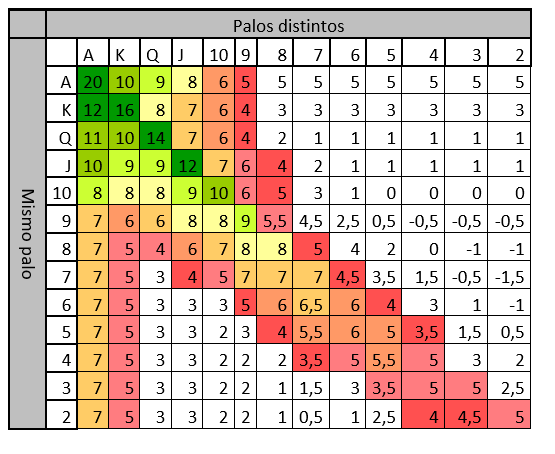
\includegraphics[width=0.8\textwidth]{figuras/chen-sklansky.png}   
\caption{Cruce de criterio de Sklansky-Malmuth con Fórmula de Chen.\cite{propiaChen}}
\label{fig:sklansky}
\end{figure}

\begin{figure}[h]
\centering
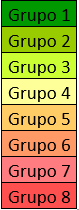
\includegraphics[width=0.1\textwidth]{figuras/grupos.png}   
\caption{Leyenda usada en la figura \ref{fig:sklansky}. \cite{propiaChen}}
\label{fig:Leyenda}
\end{figure}
